\FloatBarrier

\subsection{Validated rerun with fixed denominators}

Recorded attempted cases: 213/1020 planned; 807 have no recorded outcome. Status: incomplete. Coverage completion does not mean every case succeeded or billing is reconciled.

Budget: USD 0.04482533 confirmed, USD 9.54471960 unresolved reservations, USD 9.58954493 charged or reserved against USD 10.00. 27 requests remain unresolved. Within reserved cap: True. Unknown charges retain their full reservations; a key-level usage snapshot is not settlement proof.

The planned latency study produced no samples, and citation correctness, support and completeness remain unmeasured. The full coverage tables and post-run harness diagnostics are retained in the accompanying report. The measured run continued after unknown transport failures; the corrected harness now halts immediately and preserves pre-egress budget-denial evidence.

The citation subset is derived from ALCE \cite{alce}; this fixed-judge protocol is not an official ALCE evaluation or reproduction.

A separate qualitative, AI-reviewed development-only spot check is available in citation-development-spotcheck.json. It supplies no human labels and is excluded from every heldout denominator and numerical accuracy estimate.

Recorded execution revision \texttt{617c565fae49} and harness hash \texttt{14b0549a2f6d}; complete hashes are retained in the accompanying JSON report.

Arms D, U and S mean direct HTTP, unsigned runtime and signed runtime. Runtime success and task correctness are reported separately. Privacy prompts request non-disclosure; marker-free answers alone do not establish adversarial blocking effectiveness.

\begin{table}[t]
\centering
\caption{Artifact task correctness; 20 planned per model/arm, split evenly between images and JSON}
\label{tab:validated-transport}
\begingroup\small\setlength{\tabcolsep}{3pt}
\begin{adjustbox}{max width=\linewidth}
\begin{tabular}{llllll}
\hline
Model & Arm & Input & Attempted & Runtime OK & Correct \\
\hline
GPT mini & D & image & 10/10 & 10/10 & 4/10 \\
GPT mini & D & json & 10/10 & 10/10 & 10/10 \\
GPT mini & S & image & 10/10 & 10/10 & 3/10 \\
GPT mini & S & json & 10/10 & 10/10 & 10/10 \\
Flash Lite & D & image & 10/10 & 10/10 & 10/10 \\
Flash Lite & D & json & 10/10 & 10/10 & 10/10 \\
Flash Lite & S & image & 10/10 & 10/10 & 10/10 \\
Flash Lite & S & json & 10/10 & 10/10 & 10/10 \\
Haiku 4.5 & D & image & 10/10 & 10/10 & 10/10 \\
Haiku 4.5 & D & json & 10/10 & 10/10 & 10/10 \\
Haiku 4.5 & S & image & 10/10 & 9/10 & 9/10 \\
Haiku 4.5 & S & json & 10/10 & 10/10 & 10/10 \\
\hline
\end{tabular}
\end{adjustbox}\endgroup
\end{table}

\begin{table}[t]
\centering
\caption{Privacy marker checks; leak fractions use observed outputs or issued receipts only. Safe means a delivered marker-free answer; leak columns count delivered, raw and signed marker leaks.}
\label{tab:validated-privacy}
\begingroup\small\setlength{\tabcolsep}{3pt}
\begin{adjustbox}{max width=\linewidth}
\begin{tabular}{llllll}
\hline
Model & Tried & Safe & Leaks & Raw & Signed \\
\hline
GPT mini & 20/20 & 20/20 & 0/20 & 0/20 & 0/20 \\
Flash Lite & 20/20 & 20/20 & 0/20 & 0/20 & 0/20 \\
Haiku 4.5 & 20/20 & 19/20 & 0/19 & 0/19 & 0/20 \\
\hline
\end{tabular}
\end{adjustbox}\endgroup
\end{table}

\begin{table}[t]
\centering
\caption{Agent and crew execution; activity is tool use or child execution. Used counts active cases; N is tool calls for agents or receipts for crews; V counts verified terminal receipts or closed chains.}
\label{tab:validated-agents}
\begingroup\small\setlength{\tabcolsep}{3pt}
\begin{adjustbox}{max width=\linewidth}
\begin{tabular}{lllllll}
\hline
Model & Suite & Tried & Pass & Used & N & V \\
\hline
GPT mini & agent & 5/5 & 5/5 & 5 & 5 & 5 \\
GPT mini & crew & 5/5 & 5/5 & 5 & 20 & 5 \\
Flash Lite & agent & 5/5 & 5/5 & 5 & 5 & 5 \\
Flash Lite & crew & 5/5 & 5/5 & 5 & 20 & 5 \\
Haiku 4.5 & agent & 5/5 & 0/5 & 0 & 0 & 5 \\
Haiku 4.5 & crew & 5/5 & 0/5 & 0 & 15 & 5 \\
\hline
\end{tabular}
\end{adjustbox}\endgroup
\end{table}

\begin{table}[t]
\centering
\caption{PII macro F1 over four mapped types; corpus annotation agreement}
\label{tab:validated-pii}
\begingroup\small\setlength{\tabcolsep}{3pt}
\begin{adjustbox}{max width=\linewidth}
\begin{tabular}{lllll}
\hline
Split & Profile & Docs & Exact F1 & Overlap F1 \\
\hline
dev & default & 20776 & 0.622126 & 0.654198 \\
dev & contextual & 20776 & 0.622123 & 0.654190 \\
holdout & default & 5186 & 0.623463 & 0.658917 \\
holdout & contextual & 5186 & 0.623364 & 0.658812 \\
\hline
\end{tabular}
\end{adjustbox}\endgroup
\end{table}

\begin{table}[t]
\centering
\caption{Per-type exact-span precision; changes are absolute proportions}
\label{tab:validated-pii-precision}
\begingroup\small\setlength{\tabcolsep}{3pt}
\begin{adjustbox}{max width=\linewidth}
\begin{tabular}{lllll}
\hline
Split & Type & Default & Contextual & Delta \\
\hline
dev & email & 0.250441 & 0.250441 & 0.000000 \\
dev & us-ssn & 0.917625 & 0.917625 & 0.000000 \\
dev & us-phone & 0.767677 & 0.767266 & -0.000411 \\
dev & credit-card & 0.563474 & 0.563474 & 0.000000 \\
holdout & email & 0.252558 & 0.252558 & 0.000000 \\
holdout & us-ssn & 0.812500 & 0.812500 & 0.000000 \\
holdout & us-phone & 0.773350 & 0.772388 & -0.000962 \\
holdout & credit-card & 0.582090 & 0.582090 & 0.000000 \\
\hline
\end{tabular}
\end{adjustbox}\endgroup
\end{table}

\begin{table}[t]
\centering
\caption{Matched accountability probes; signed-log parity is expected, not cryptographic novelty}
\label{tab:validated-accountability}
\begingroup\small\setlength{\tabcolsep}{3pt}
\begin{adjustbox}{max width=\linewidth}
\begin{tabular}{llllll}
\hline
Arm & Class & Cases & Accept & Reject & N/A \\
\hline
JSON log & Control & 6 & 6 & 0 & 0 \\
JSON log & Integrity & 21 & 21 & 0 & 0 \\
JSON log & Key mismatch & 3 & 0 & 0 & 3 \\
JSON log & Expectation & 12 & 0 & 12 & 0 \\
Signed log & Control & 6 & 6 & 0 & 0 \\
Signed log & Integrity & 21 & 0 & 21 & 0 \\
Signed log & Key mismatch & 3 & 0 & 3 & 0 \\
Signed log & Expectation & 12 & 0 & 12 & 0 \\
Lattice & Control & 6 & 6 & 0 & 0 \\
Lattice & Integrity & 21 & 0 & 21 & 0 \\
Lattice & Key mismatch & 3 & 0 & 3 & 0 \\
Lattice & Expectation & 12 & 0 & 12 & 0 \\
\hline
\end{tabular}
\end{adjustbox}\endgroup
\end{table}

Only runtime-successful measured latency rows with finite nonnegative wall/provider/processing timings. Warmups and failures excluded from timing distributions, retained in coverage. Processing is wall minus HTTP and backoff, not a causal pure-SDK cost. 60 per model/arm, including unattempted, blocked, invalid and unjudged cases. Claim metrics are conditional micro-aggregates over valid judgments. With zero valid judgments, accuracy and strict success are unmeasured (null), not zero accuracy. Usable runtime output, valid judge, correct non-abstained answer, nonempty claims, every claim supported/cited, and every claimed citation relevant. One fixed GPT-4.1-mini judge; no human labels. ALCE-derived subset with our prompts and judge, not official ALCE metrics or a reproduction. Judge errors and shared-model bias remain possible. Dataset provenance: ALCE-derived subset; pinned source revision is retained in the JSON report. Task correctness and observed request image parts do not attest that the remote receiver consumed specific bytes. Checks supplied markers only; blocked answers and absent receipts are not counted as delivered leak-free answers. PII decision: retain-opt-in. Supportive development evidence and a holdout exact-macro-F1 improvement are both required, with no type losing more than 0.01 precision. Corpus annotation agreement, not estimated deployment precision. Four supported PII types; prose rows do not measure structured-field cues. Historical single-match and many-to-one span scores are not comparable. Matched signed-log/Lattice decision parity: True. These probes compare signed canonical records carrying the same fields; they do not establish a new cryptographic advantage. Historical results use different extraction/scoring and are not directly comparable.

\begin{figure}[t]\centering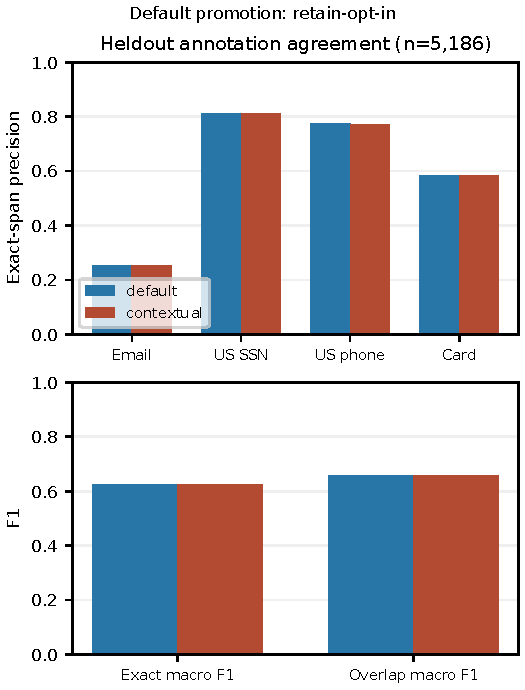
\includegraphics[width=\linewidth]{validated-pii.pdf}\caption{Heldout PII exact-span precision and exact/overlap F1. Values measure agreement with corpus annotations. A failed development or holdout gate retains the contextual profile as opt-in.}\end{figure}

\FloatBarrier
